% Fig. 3, Method (v3 architecture diagram). Source: paper/figures/cvpr_v1/fig03_pipeline.pdf (+ .json sidecar).
\begin{figure*}[t]
\centering
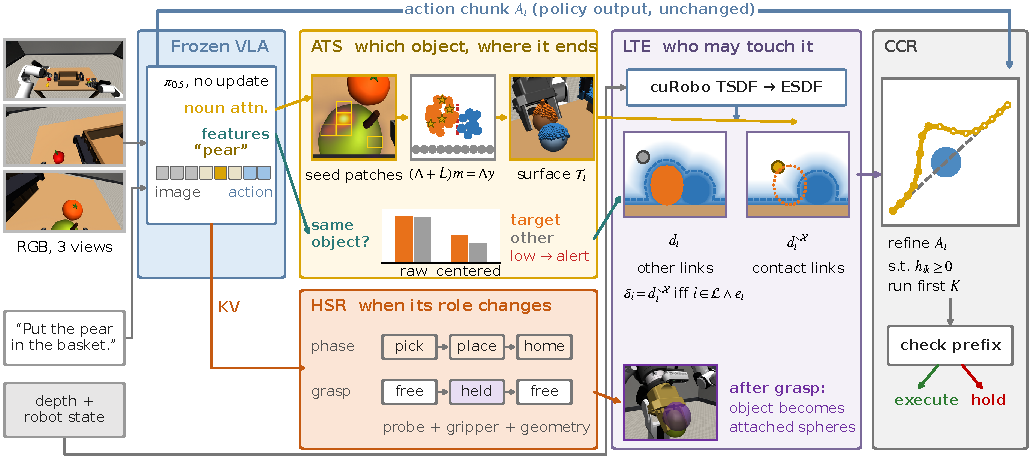
\includegraphics[width=\textwidth]{../figures/cvpr_v1/fig03_pipeline.pdf}
\caption{\textbf{Method overview.} The frozen VLA produces the action chunk unchanged; an instrumented copy exposes noun attention, patch features, and key/value features. \textbf{ATS} (Secs.~\ref{sec:grounding}--\ref{sec:memory}) seeds a depth-continuous surface graph from the attention patches; edges never cross a depth break (red), support nodes are negative evidence, and the membership solve of Eq.~\eqref{eq:energy} yields the target's observed surface. Centered features compare the selection with the remembered object and raise an alert when agreement drops. \textbf{HSR} (Sec.~\ref{sec:phase}) tracks the task phase and, separately, the physical grasp state. \textbf{LTE} (Sec.~\ref{sec:contact}) builds the cuRobo TSDF/ESDF scene field and a second field without the accepted target surface; only contact links read the second, while the neighbor stays an obstacle in both, and after a confirmed grasp the object is carried as attached spheres. \textbf{CCR} (Sec.~\ref{sec:refine}) refines the chunk under the clearance constraints of Eq.~\eqref{eq:clearance} and executes the checked prefix or holds. The field slices are an exact 2-D distance transform of a synthetic cross-section; the graph and refinement panels are schematic; the remaining panels are recorded frames.}
\label{fig:pipeline}
\end{figure*}
